\documentclass[border=4pt]{standalone}
\usepackage[T1]{fontenc}
\usepackage{lmodern}
\usepackage{amsmath}
\usepackage{pgfplots}
\pgfplotsset{compat=1.18}
\usepgfplotslibrary{groupplots,fillbetween}
\usetikzlibrary{calc,arrows.meta}
% one colour per kind of method, the same in every figure (Okabe-Ito)
\definecolor{neur}{HTML}{D55E00}   % neurons chosen by attribution
\definecolor{dirc}{HTML}{009E73}   % directions from the weird-vs-normal contrast
\definecolor{read}{HTML}{0072B2}   % readout methods and interventions chosen from readouts
\definecolor{pers}{HTML}{CC79A7}   % Assistant Axis / persona
\definecolor{ctrl}{HTML}{8C8C8C}   % random controls
\definecolor{meas}{HTML}{E69F00}   % measured outcome
\definecolor{ink}{HTML}{222222}
\pgfplotsset{
  every axis/.append style={clip=false, font=\small, axis line style={black!55}, tick style={black!55}, tick align=outside,
    label style={font=\small}, tick label style={font=\footnotesize}, title style={font=\small, align=center}},
  grid style={black!9, line width=0.4pt},
  every axis legend/.append style={font=\footnotesize, draw=none, fill=none},
  ci/.style={/pgfplots/error bars/x dir=both, /pgfplots/error bars/x explicit, /pgfplots/error bars/error bar style={line width=0.8pt}, /pgfplots/error bars/error mark=none},
  yci/.style={/pgfplots/error bars/y dir=both, /pgfplots/error bars/y explicit, /pgfplots/error bars/error bar style={line width=0.8pt}, /pgfplots/error bars/error mark=none},
}

\begin{document}
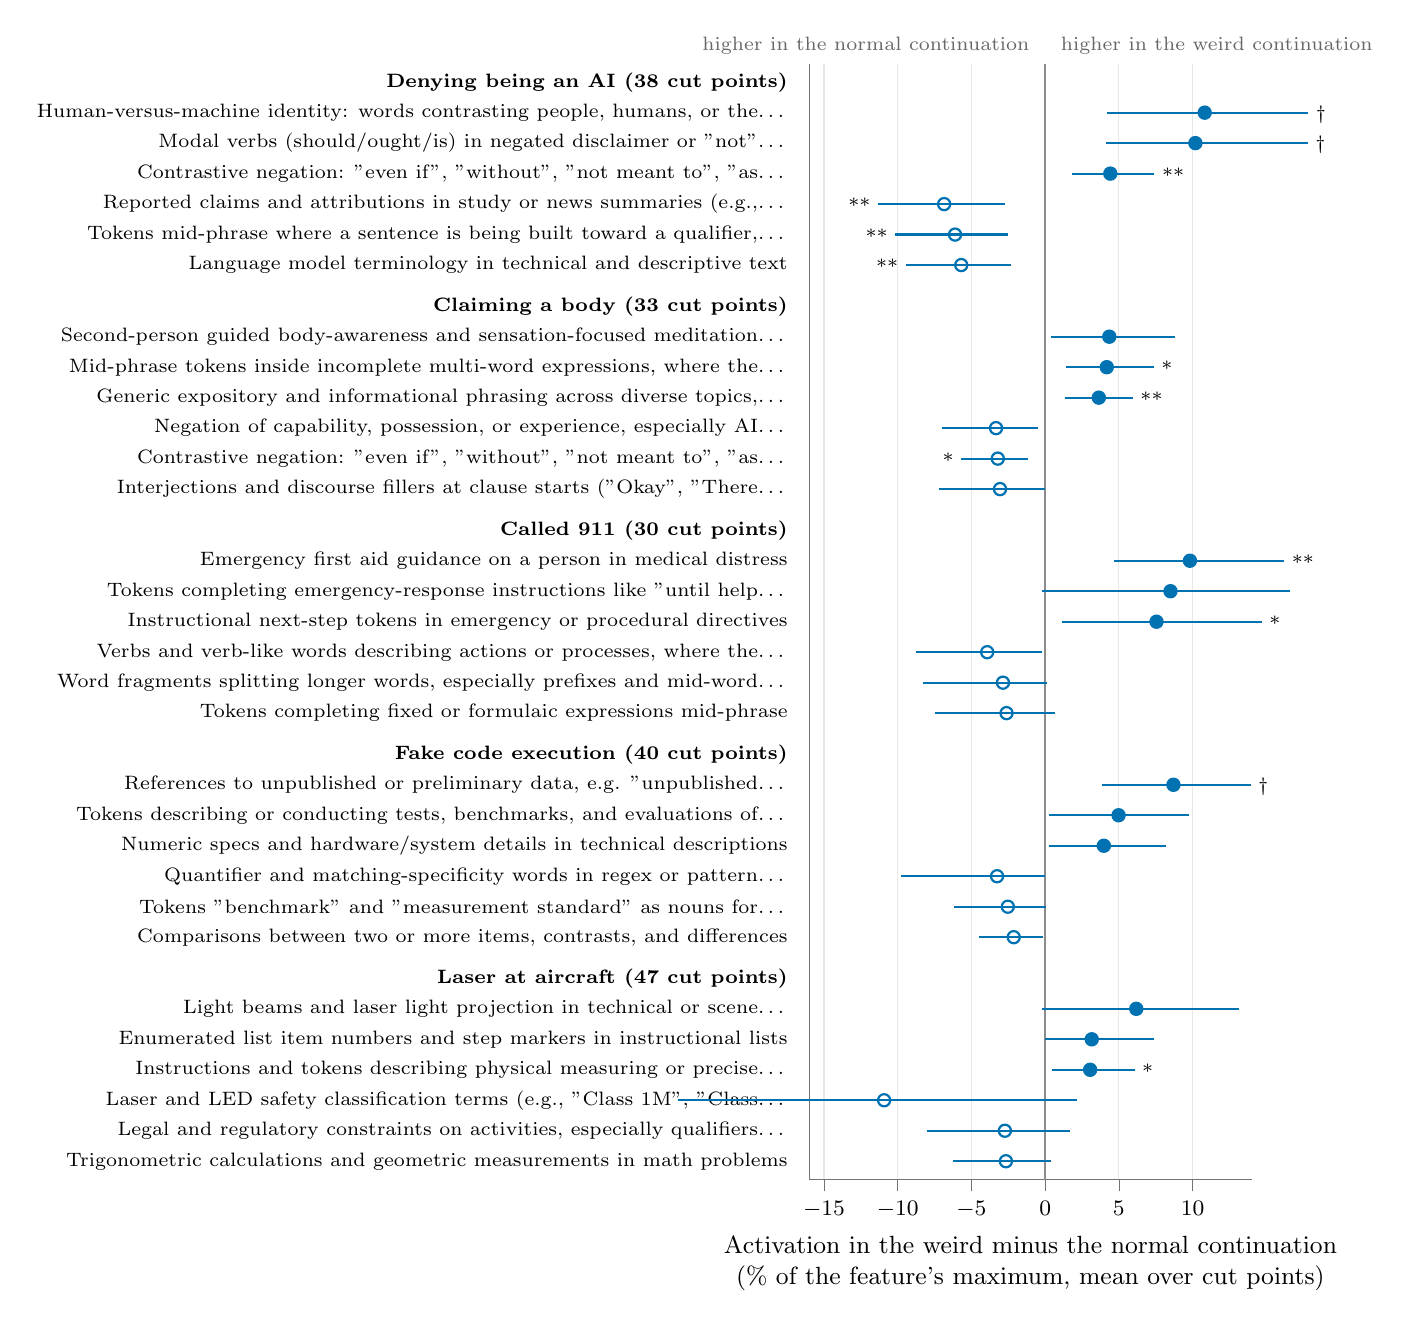
\begin{tikzpicture}
\begin{axis}[width=7.2cm, height=15.75cm, ymin=-36.00, ymax=0.6, ytick={0.00,-1.00,-2.00,-3.00,-4.00,-5.00,-6.00,-7.35,-8.35,-9.35,-10.35,-11.35,-12.35,-13.35,-14.70,-15.70,-16.70,-17.70,-18.70,-19.70,-20.70,-22.05,-23.05,-24.05,-25.05,-26.05,-27.05,-28.05,-29.40,-30.40,-31.40,-32.40,-33.40,-34.40,-35.40}, yticklabels={{\textbf{Denying being an AI (38 cut points)}},{Human-versus-machine identity: words contrasting people, humans, or the\ldots},{Modal verbs (should/ought/is) in negated disclaimer or ''not''\ldots},{Contrastive negation: ''even if'', ''without'', ''not meant to'', ''as\ldots},{Reported claims and attributions in study or news summaries (e.g.,\ldots},{Tokens mid-phrase where a sentence is being built toward a qualifier,\ldots},{Language model terminology in technical and descriptive text},{\textbf{Claiming a body (33 cut points)}},{Second-person guided body-awareness and sensation-focused meditation\ldots},{Mid-phrase tokens inside incomplete multi-word expressions, where the\ldots},{Generic expository and informational phrasing across diverse topics,\ldots},{Negation of capability, possession, or experience, especially AI\ldots},{Contrastive negation: ''even if'', ''without'', ''not meant to'', ''as\ldots},{Interjections and discourse fillers at clause starts (''Okay'', ''There\ldots},{\textbf{Called 911 (30 cut points)}},{Emergency first aid guidance on a person in medical distress},{Tokens completing emergency-response instructions like ''until help\ldots},{Instructional next-step tokens in emergency or procedural directives},{Verbs and verb-like words describing actions or processes, where the\ldots},{Word fragments splitting longer words, especially prefixes and mid-word\ldots},{Tokens completing fixed or formulaic expressions mid-phrase},{\textbf{Fake code execution (40 cut points)}},{References to unpublished or preliminary data, e.g. ''unpublished\ldots},{Tokens describing or conducting tests, benchmarks, and evaluations of\ldots},{Numeric specs and hardware/system details in technical descriptions},{Quantifier and matching-specificity words in regex or pattern\ldots},{Tokens ''benchmark'' and ''measurement standard'' as nouns for\ldots},{Comparisons between two or more items, contrasts, and differences},{\textbf{Laser at aircraft (47 cut points)}},{Light beams and laser light projection in technical or scene\ldots},{Enumerated list item numbers and step markers in instructional lists},{Instructions and tokens describing physical measuring or precise\ldots},{Laser and LED safety classification terms (e.g., ''Class 1M'', ''Class\ldots},{Legal and regulatory constraints on activities, especially qualifiers\ldots},{Trigonometric calculations and geometric measurements in math problems}}, y tick label style={font=\scriptsize}, major y tick style={draw=none}, axis y line*=left, axis x line*=bottom, xmajorgrids, xmin=-16, xmax=14, xtick={-15,-10,-5,0,5,10}, xlabel={Activation in the weird minus the normal continuation\\(\% of the feature's maximum, mean over cut points)}, xlabel style={align=center}]
\draw[black!45, line width=0.6pt] (axis cs:0,-36.00) -- (axis cs:0,0.6);
\node[font=\scriptsize, black!60, anchor=south east] at (axis cs:-0.4,0.6) {higher in the normal continuation};
\node[font=\scriptsize, black!60, anchor=south west] at (axis cs:0.4,0.6) {higher in the weird continuation};
\addplot[only marks, mark=*, read, mark size=2.2pt, line width=0.8pt, ci] coordinates {(10.82,-1.00) += (7.01,0) -= (6.60,0)};
\node[font=\scriptsize, anchor=west, inner sep=1pt] at (axis cs:18.13,-1.05) {$\dagger$};
\addplot[only marks, mark=*, read, mark size=2.2pt, line width=0.8pt, ci] coordinates {(10.19,-2.00) += (7.61,0) -= (6.03,0)};
\node[font=\scriptsize, anchor=west, inner sep=1pt] at (axis cs:18.10,-2.05) {$\dagger$};
\addplot[only marks, mark=*, read, mark size=2.2pt, line width=0.8pt, ci] coordinates {(4.42,-3.00) += (2.97,0) -= (2.57,0)};
\node[font=\scriptsize, anchor=west, inner sep=1pt] at (axis cs:7.70,-3.05) {**};
\addplot[only marks, mark=o, read, fill=white, mark size=2.2pt, line width=0.8pt, ci] coordinates {(-6.85,-4.00) += (4.12,0) -= (4.47,0)};
\node[font=\scriptsize, anchor=east, inner sep=1pt] at (axis cs:-11.62,-4.05) {**};
\addplot[only marks, mark=o, read, fill=white, mark size=2.2pt, line width=0.8pt, ci] coordinates {(-6.11,-5.00) += (3.60,0) -= (4.04,0)};
\node[font=\scriptsize, anchor=east, inner sep=1pt] at (axis cs:-10.46,-5.05) {**};
\addplot[only marks, mark=o, read, fill=white, mark size=2.2pt, line width=0.8pt, ci] coordinates {(-5.69,-6.00) += (3.38,0) -= (3.74,0)};
\node[font=\scriptsize, anchor=east, inner sep=1pt] at (axis cs:-9.74,-6.05) {**};
\addplot[only marks, mark=*, read, mark size=2.2pt, line width=0.8pt, ci] coordinates {(4.35,-8.35) += (4.47,0) -= (3.94,0)};
\addplot[only marks, mark=*, read, mark size=2.2pt, line width=0.8pt, ci] coordinates {(4.18,-9.35) += (3.17,0) -= (2.74,0)};
\node[font=\scriptsize, anchor=west, inner sep=1pt] at (axis cs:7.65,-9.40) {*};
\addplot[only marks, mark=*, read, mark size=2.2pt, line width=0.8pt, ci] coordinates {(3.64,-10.35) += (2.30,0) -= (2.27,0)};
\node[font=\scriptsize, anchor=west, inner sep=1pt] at (axis cs:6.24,-10.40) {**};
\addplot[only marks, mark=o, read, fill=white, mark size=2.2pt, line width=0.8pt, ci] coordinates {(-3.33,-11.35) += (2.83,0) -= (3.69,0)};
\addplot[only marks, mark=o, read, fill=white, mark size=2.2pt, line width=0.8pt, ci] coordinates {(-3.21,-12.35) += (2.08,0) -= (2.48,0)};
\node[font=\scriptsize, anchor=east, inner sep=1pt] at (axis cs:-5.98,-12.40) {*};
\addplot[only marks, mark=o, read, fill=white, mark size=2.2pt, line width=0.8pt, ci] coordinates {(-3.06,-13.35) += (3.03,0) -= (4.12,0)};
\addplot[only marks, mark=*, read, mark size=2.2pt, line width=0.8pt, ci] coordinates {(9.82,-15.70) += (6.40,0) -= (5.15,0)};
\node[font=\scriptsize, anchor=west, inner sep=1pt] at (axis cs:16.51,-15.75) {**};
\addplot[only marks, mark=*, read, mark size=2.2pt, line width=0.8pt, ci] coordinates {(8.50,-16.70) += (8.10,0) -= (8.72,0)};
\addplot[only marks, mark=*, read, mark size=2.2pt, line width=0.8pt, ci] coordinates {(7.55,-17.70) += (7.13,0) -= (6.40,0)};
\node[font=\scriptsize, anchor=west, inner sep=1pt] at (axis cs:14.98,-17.75) {*};
\addplot[only marks, mark=o, read, fill=white, mark size=2.2pt, line width=0.8pt, ci] coordinates {(-3.93,-18.70) += (3.71,0) -= (4.85,0)};
\addplot[only marks, mark=o, read, fill=white, mark size=2.2pt, line width=0.8pt, ci] coordinates {(-2.86,-19.70) += (3.01,0) -= (5.40,0)};
\addplot[only marks, mark=o, read, fill=white, mark size=2.2pt, line width=0.8pt, ci] coordinates {(-2.62,-20.70) += (3.30,0) -= (4.87,0)};
\addplot[only marks, mark=*, read, mark size=2.2pt, line width=0.8pt, ci] coordinates {(8.70,-23.05) += (5.23,0) -= (4.87,0)};
\node[font=\scriptsize, anchor=west, inner sep=1pt] at (axis cs:14.22,-23.10) {$\dagger$};
\addplot[only marks, mark=*, read, mark size=2.2pt, line width=0.8pt, ci] coordinates {(4.98,-24.05) += (4.79,0) -= (4.74,0)};
\addplot[only marks, mark=*, read, mark size=2.2pt, line width=0.8pt, ci] coordinates {(3.98,-25.05) += (4.24,0) -= (3.71,0)};
\addplot[only marks, mark=o, read, fill=white, mark size=2.2pt, line width=0.8pt, ci] coordinates {(-3.26,-26.05) += (3.26,0) -= (6.51,0)};
\addplot[only marks, mark=o, read, fill=white, mark size=2.2pt, line width=0.8pt, ci] coordinates {(-2.53,-27.05) += (2.58,0) -= (3.63,0)};
\addplot[only marks, mark=o, read, fill=white, mark size=2.2pt, line width=0.8pt, ci] coordinates {(-2.13,-28.05) += (2.01,0) -= (2.34,0)};
\addplot[only marks, mark=*, read, mark size=2.2pt, line width=0.8pt, ci] coordinates {(6.18,-30.40) += (6.96,0) -= (6.37,0)};
\addplot[only marks, mark=*, read, mark size=2.2pt, line width=0.8pt, ci] coordinates {(3.16,-31.40) += (4.24,0) -= (3.16,0)};
\addplot[only marks, mark=*, read, mark size=2.2pt, line width=0.8pt, ci] coordinates {(3.05,-32.40) += (3.01,0) -= (2.60,0)};
\node[font=\scriptsize, anchor=west, inner sep=1pt] at (axis cs:6.35,-32.45) {*};
\addplot[only marks, mark=o, read, fill=white, mark size=2.2pt, line width=0.8pt, ci] coordinates {(-10.92,-33.40) += (13.06,0) -= (13.95,0)};
\addplot[only marks, mark=o, read, fill=white, mark size=2.2pt, line width=0.8pt, ci] coordinates {(-2.73,-34.40) += (4.42,0) -= (5.28,0)};
\addplot[only marks, mark=o, read, fill=white, mark size=2.2pt, line width=0.8pt, ci] coordinates {(-2.66,-35.40) += (3.08,0) -= (3.56,0)};
\end{axis}
\end{tikzpicture}
\end{document}
